\documentclass[aspectratio=169]{beamer}
\usetheme{Madrid}
\usecolortheme{beaver}
\usepackage[utf8]{inputenc}
\usepackage[T1]{fontenc}
\usepackage{tikz}
\usepackage{amssymb}
\usepackage{graphicx}
\setbeamertemplate{navigation symbols}{}
\setbeamercolor{title}{fg=white,bg=cyan!60!black}
\setbeamercolor{frametitle}{fg=white,bg=cyan!50!black}
\setbeamercolor{block title}{bg=cyan!15,fg=black}
\setbeamercolor{block body}{bg=cyan!5,fg=black}

\title{Block Arcade 1 — Sprites \& the Stage}
\subtitle{Lesson 1: Meet Your Sprite}
\author{ByteForge --- Grade 7 --- Game Maker}
\date{}

\begin{document}

\begin{frame}
    \titlepage
\end{frame}

\begin{frame}{A sprite is just a shape at a position}
    \Large
    A "sprite" is any character or object on the stage — under the hood, it's a position (x, y) plus something drawn there.

    \begin{center}
    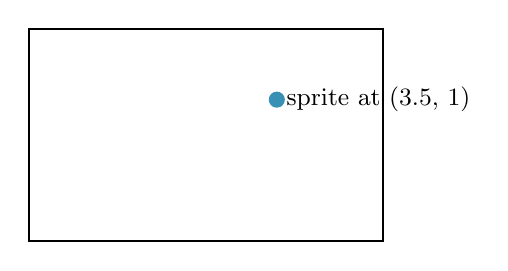
\begin{tikzpicture}[scale=0.9]

        \draw[thick] (0,0) rectangle (5,-3);
        \filldraw[cyan!70!black] (3.5,-1) circle (3pt);
        \node[right] at (3.5,-1) {\small sprite at (3.5, 1)};
    \end{tikzpicture}
    \end{center}
\end{frame}

\begin{frame}{Your Turn}
    \Large
    Open the student map, find \textbf{Block Arcade 1 — Sprites \& the Stage}, and complete
    the \textbf{Meet Your Sprite} challenge --- everything you just saw, they now do themselves.
\end{frame}

\end{document}
